% Created 2022-05-29 Sun 21:43
% Intended LaTeX compiler: pdflatex
\documentclass[presentation,aspectratio=169]{beamer}
\usepackage[utf8]{inputenc}
\usepackage[T1]{fontenc}
\usepackage{graphicx}
\usepackage{grffile}
\usepackage{longtable}
\usepackage{wrapfig}
\usepackage{rotating}
\usepackage[normalem]{ulem}
\usepackage{amsmath}
\usepackage{textcomp}
\usepackage{amssymb}
\usepackage{capt-of}
\usepackage{hyperref}
\usepackage{khpreamble}
\usepackage{amssymb}
\usepgfplotslibrary{groupplots}
\newcommand*{\shift}{\operatorname{q}}
\DeclareMathSymbol{\Omega}{\mathalpha}{letters}{"0A}% italics
\DeclareMathSymbol{\varOmega}{\mathalpha}{operators}{"0A}% upright
\providecommand*{\upOmega}{\varOmega}% for siunitx
\usepackage[binary-units=true]{siunitx}
\usepackage{circuitikz}
\usetikzlibrary{calc}
\usetheme{default}
\author{Kjartan Halvorsen}
\date{2022-05-30}
\title{State-space models  - stability}
\hypersetup{
 pdfauthor={Kjartan Halvorsen},
 pdftitle={State-space models  - stability},
 pdfkeywords={},
 pdfsubject={},
 pdfcreator={Emacs 26.3 (Org mode 9.4.6)}, 
 pdflang={English}}
\begin{document}

\maketitle

\section{Modelo compartamental}
\label{sec:org4236504}

\begin{frame}[label={sec:org8b776f0}]{Compartment model}
 \small
\begin{columns}
  \begin{column}{0.5\linewidth}
    \begin{center}
      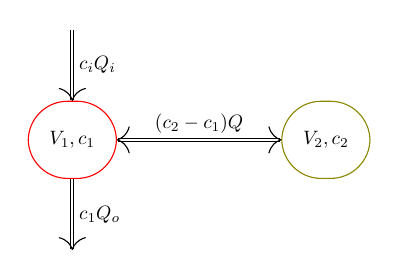
\begin{tikzpicture}[scale=0.7, transform shape,
	compartment/.style={rounded corners=5mm, minimum height=14mm, minimum width=16mm},
	node distance=46mm,
	]

	\node[compartment, draw=red, ] (comp1) {$V_1, c_1$};
	\node[compartment, right of=comp1, draw=olive,] (comp2) {$V_2, c_2$};

	\node[coordinate, above of=comp1, node distance=20mm] (input) {};
	\node[coordinate, below of=comp1, node distance=20mm] (output) {};

	\draw[->, double] (input) -- node[right]{$c_{i}Q_i$} (comp1);
	\draw[->, double] (comp1) -- node[right]{$c_{1}Q_o$} (output);
	\draw[<->, double] (comp1) -- node[above]{$(c_{2}-c_1)Q$} (comp2);

      \end{tikzpicture}
    \end{center}

  \end{column}
  \begin{column}{0.5\linewidth}
    \begin{equation*}
      \begin{aligned}
	V_1\frac{dc_1}{dt} &= Q(c_2-c_1) - Q_{o}c_1 + Q_ic_{i}, \quad  & c_1 \geq 0 \\
	V_2\frac{dc_2}{dt} &= Q(c_1-c_2),  & c_2 \geq 0,
      \end{aligned}
    \end{equation*}
  \end{column}
\end{columns}

\begin{center}
\Large
\begin{align*}
  \dot{x} &= \overbrace{\begin{bmatrix} \textcolor{white}{-\frac{Q+Q_o}{V_1}}  & \textcolor{white}{\frac{Q}{V_1}}\\
              \textcolor{white}{\frac{Q}{V_2}}  & \textcolor{white}{-\frac{Q}{V_2}}\end{bmatrix}}^A \begin{bmatrix} {x_1}\\ {x_2}\end{bmatrix}  + \overbrace{\begin{bmatrix} \textcolor{white}{\frac{1}{V_1}} \\ \textcolor{white}{0} \end{bmatrix}}^B  u \\
       y &=  \underbrace{\begin{bmatrix} \textcolor{white}{1} &  \textcolor{white}{0}\end{bmatrix}}_C \begin{bmatrix} x_1\\ x_2\end{bmatrix}
\end{align*}

\end{center}
\end{frame}

\begin{frame}[label={sec:org6cb8f34}]{Compartment model}
 \small
\begin{columns}
  \begin{column}{0.5\linewidth}
    \begin{center}
      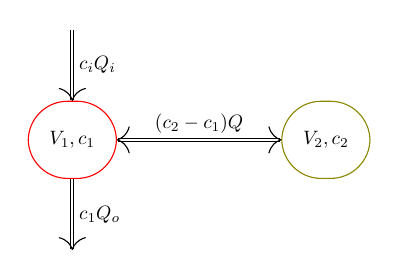
\begin{tikzpicture}[scale=0.7, transform shape,
	compartment/.style={rounded corners=5mm, minimum height=14mm, minimum width=16mm},
	node distance=46mm,
	]

	\node[compartment, draw=red, ] (comp1) {$V_1, c_1$};
	\node[compartment, right of=comp1, draw=olive,] (comp2) {$V_2, c_2$};

	\node[coordinate, above of=comp1, node distance=20mm] (input) {};
	\node[coordinate, below of=comp1, node distance=20mm] (output) {};

	\draw[->, double] (input) -- node[right]{$c_{i}Q_i$} (comp1);
	\draw[->, double] (comp1) -- node[right]{$c_{1}Q_o$} (output);
	\draw[<->, double] (comp1) -- node[above]{$(c_{2}-c_1)Q$} (comp2);

      \end{tikzpicture}
    \end{center}

  \end{column}
  \begin{column}{0.5\linewidth}
    \begin{equation*}
      \begin{aligned}
	V_1\frac{dc_1}{dt} &= Q(c_2-c_1) - Q_{o}c_1 + Q_ic_{i}, \quad  & c_1 \geq 0 \\
	V_2\frac{dc_2}{dt} &= Q(c_1-c_2),  & c_2 \geq 0,
      \end{aligned}
    \end{equation*}
  \end{column}
\end{columns}

\begin{center}
\Large
\begin{align*}
  \dot{x} &= \overbrace{\begin{bmatrix} \textcolor{red!80!black}{-\frac{Q+Q_o}{V_1}}  & \textcolor{red!80!black}{\frac{Q}{V_1}}\\
              \textcolor{red!80!black}{\frac{Q}{V_2}}  & \textcolor{red!80!black}{-\frac{Q}{V_2}}\end{bmatrix}}^A \begin{bmatrix} {x_1}\\ {x_2}\end{bmatrix}  + \overbrace{\begin{bmatrix} \textcolor{red!80!black}{\frac{1}{V_1}} \\ \textcolor{red!80!black}{0} \end{bmatrix}}^B  u \\
       y &=  \underbrace{\begin{bmatrix} \textcolor{red!80!black}{1} &  \textcolor{red!80!black}{0}\end{bmatrix}}_C \begin{bmatrix} x_1\\ x_2\end{bmatrix}
\end{align*}

\end{center}
\end{frame}


\begin{frame}[label={sec:org2134300}]{Homogeneous solution}
\footnotesize
   \[\dot{x} &= Ax, \qquad x(0) = x_0\]

\pause

\begin{columns}
\begin{column}{0.5\columnwidth}
\begin{block}{The matrix exponential}
There exists a function \(\Phi:\, \mathbb{R} \mapsto \mathbb{R}^{n\times n}\) \[\Phi(t)=\mathrm{e}^{At} = I + tA + \frac{t^2}{2!}A^2 + \frac{t^3}{3!}A^3 + \cdots\] that has the property
\[\dot{\Phi} = A\Phi, \quad \Phi(0) = I.\]

\pause

The homogeneous solution to the state-space model is
   \[ x(t) = \Phi(t)x(0)\]

\pause
\end{block}
\end{column}

\begin{column}{0.5\columnwidth}
\begin{block}{Eigenvalues and eigenvectors}
If the initial value \(x(0) = v\) is an eigenvector of the matrix \(A\)
\[ Av = \lambda v,\]
\begin{align*}
 x(t) &= \Phi(t) v = \mathrm{e}^{At}v\\ &= (I + tA + \frac{t^2}{2!}A^2 + \frac{t^3}{3!}A^3 + \cdots) v\\
      &= Iv + tAv + \frac{t^2}{2!}A^2v + \frac{t^3}{3!}A^3v + \cdots\\ &= v + t\lambda v + \frac{(t\lambda)^2}{2!}v + \frac{(t\lambda)^3}{3!}v + \cdots\\
      &= \mathrm{e}^{\lambda t} v 
\end{align*}
\end{block}
\end{column}
\end{columns}
\end{frame}

\begin{frame}[label={sec:orgd28113a}]{Stability}
Stability is a key property of the system itself. It does not depend on the input signal.

The homogeneous solution can be written
   \[ x(t) = \mathrm{e}^{\lambda_1 t}\alpha_1v_1 + \mathrm{e}^{\lambda_2 t}\alpha_2v_2 + \cdots + \mathrm{e}^{\lambda_n t}\alpha_nv_n.\]

\pause

Stability requires that \alert{each} of the exponential functions go to zero.

\pause

\begin{center}
A sufficient and necessary condition is that \emph{all} the eigenvalues of $A$ has negative real-part. \[ \mathrm{Re}\{\lambda_i\} < 0, \; \forall i=1,2,3\ldots, n\]
\end{center}

The eigenvalues of \(A\) are the \alert{poles} of the system.
\end{frame}
\end{document}